The $VH$ production mode has already been observed in the $H \to b\bar{b}$ decay channel, and our Run~3 \hww{} analysis is expected to measure the signal yield in this channel with good accuracy. While one of our primary goals is to reach a $5\sigma$ observation, it is also important to extract the production cross sections for both the \wh{} and \zh{} modes, as well as perform differential cross-section measurements. This differential measurement could be done using any number of variables such as jet multiplicity or rapidity of the associated vector boson, but instead will be performed using the \pt{} of the associated vector boson. Given the anticipated $5\sigma$ sensitivity expected with just the Run~3 data, the number and type of observables and bins is limited. Special attention must be given to ensure compatibility with other ATLAS analyses, as well as potential future combinations with CMS, meaning that variable choices and binning must align with ongoing and upcoming harmonization efforts within and across experiments.

This work has been conducted within the LHC Higgs Cross Section Working Group and has contributed to a series of recommendations defining key observables and their binning schemes for differential cross-section measurements. These recommendations are part of the Simplified Template Cross Sections (STXS) framework, which was developed to enable consistent and interpretable measurements of Higgs boson production across experiments and theory. The STXS framework divides phase space into distinct regions (bins) based on the kinematics of the Higgs boson and associated particles. The regions are organized into different ``stages'', each corresponding to a specific binning configuration that balances physical interest and analysis selection requirements. The binning becomes increasingly granular with higher stage numbers, allowing for more refined measurements when the available dataset provides sufficient statistical significance in individual bins.

For the present analysis, we will use the binning configuration defined in Stage 1.2~\cite{Berger:2922392}, as illustrated in Figure~\ref{fig:stxs_12_figure}. While alternative binning configurations exist for other Higgs production modes beyond $VH$, they are not relevant to this discussion and are therefore omitted.

\begin{figure}[htbp]
    \centering
    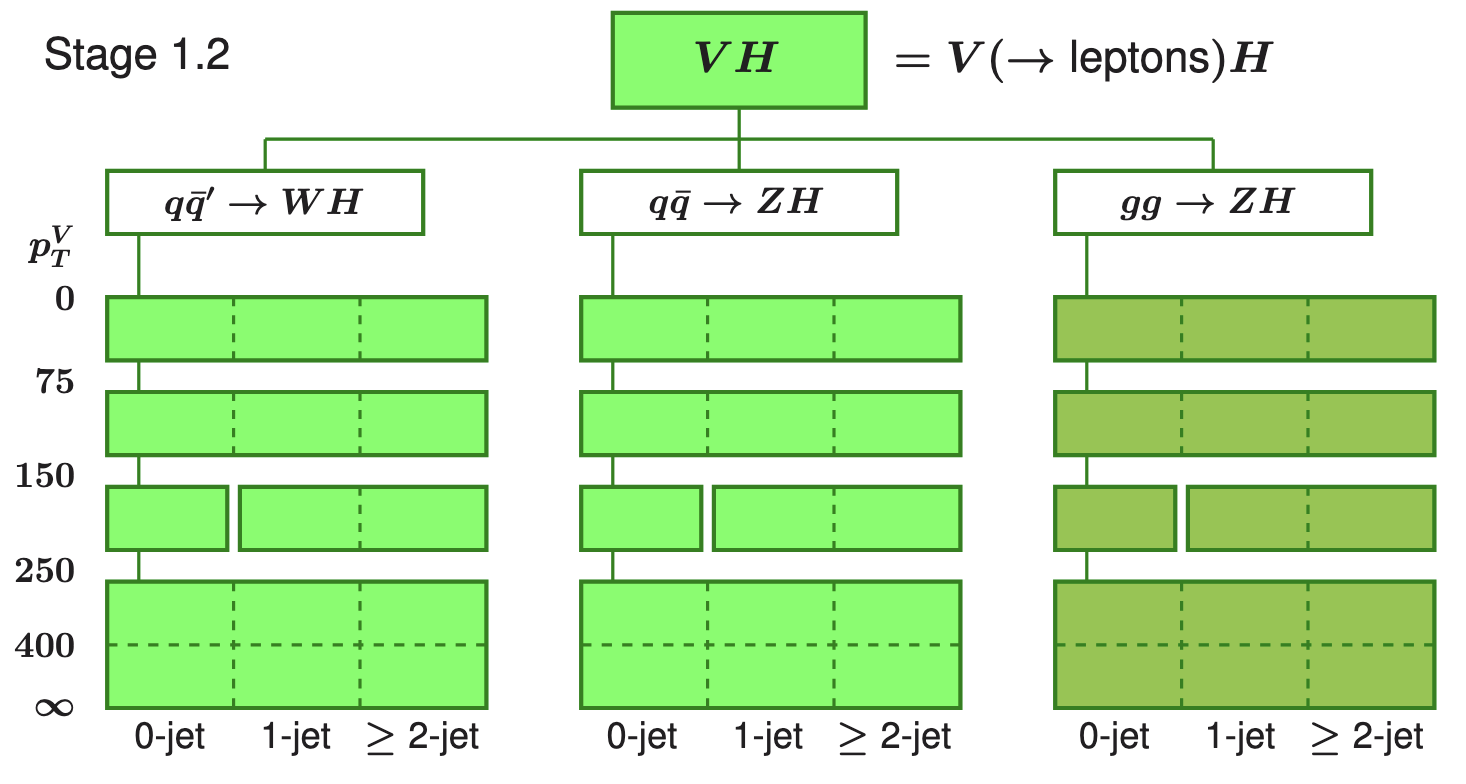
\includegraphics[width=1\textwidth]{figures/stxs/stxs_stxs_1_2.png}
    \caption{The Stage 1.2 binning configuration for the $VH$ production mode, as defined by the LHC Higgs Cross Section Working Group~\cite{Berger:2922392}.}\label{fig:stxs_12_figure}
\end{figure}

In Figure~\ref{fig:stxs_12_figure}, two types of divisions are visible: those marked with dashed lines and those separated by white space. The dashed lines represent the bin boundaries used to split the MC samples during the analysis. These divisions are used for incorporating theoretical uncertainties that impact the shape of some observables, such as variations in the predicted yield and migrations between bins. In contrast, the white space divisions indicate the recommended bins for measurement.

The measured cross sections here are defined on the basis of available statistics. It is not useful for us to split our STXS regions by number of jets, nor split the 150--400 GeV \pt{} bin, due to the limited statistics available. Therefore our measurements will be conducted in three \pt{} bins: 0--75~GeV, 75--150~GeV, and 150+~GeV, and fully inclusive in jets. 
